%%%%%%%%%%%%%%%%%%%%%%%%%%%%%%%%%%%%%%%
%%  MISCELLANEOUS SETTINGS/COMMANDS  %%
%%%%%%%%%%%%%%%%%%%%%%%%%%%%%%%%%%%%%%%


\newcommand{\balA}[1][1]{BAL$^\mathup{I}_{#1:#1}$\xspace}
\newcommand{\unbalA}[1][n]{UNBAL$^\mathup{I}_{1:#1}$\xspace}
\newcommand{\balB}[1][1]{BAL$^\mathup{II}_{#1:#1}$\xspace}
\newcommand{\unbalB}[1][n]{UNBAL$^\mathup{II}_{#1:1}$\xspace}

% Add separator slide to the beginning of each section ==>
%% Blue on white:
%\AtBeginSection[]{%
%	\begin{frame}[standout, c]{~}
%		%\vfill
%		\usebeamerfont{title}%
%		\textcolor{SpotColor}{\insertsectionhead}
%		%\vfill
%	\end{frame}%
%}
% White on blue:
\AtBeginSection[]{{%
	\setbeamercolor{background canvas}{bg=UBonnBlue, fg=white}%
	\colorlet{SpotColor}{white}%
	\begin{frame}[standout, c]{~}
		%\vfill
		\usebeamerfont{title}\hypersetup{linkcolor=white}%
		\insertsection
		%\vfill
	\end{frame}%
	\colorlet{SpotColor}{UBonnBlue}%
}}
%% Alternativelyy, add ``Outline'' slide to the beginning of each section ==>
%\AtBeginSection[]{
%	\begin{frame}[plain]{Outline}
%		\tableofcontents[currentsection]
%	\end{frame}
%}
%% <==

\title{Academic Presentations}

\subtitle{A~LaTeX Template Using the \texttt{beamer} Class}

%\subtitle{I~Prefer to Avoid Subtitles}

\author[Smith, Smith, and Smith]{%
	Adam Smith\inst{a,\,c} \and
	% Set the name of the presenting coauthor in boldface:
	\alert{Janet Smith}\inst{b,\,c} \and
	Jeremiah Smith\inst{a}
} % Author(s)

\institute{%
	\inst{a}\,University of Bonn, Germany \and
	\inst{b}\,University of Cologne, Germany \and
	\inst{c}\,Collaborative Research Center Transregio~224%
} % Institution(s)

\date{%
	Name of the Inviting Institution/Seminar Series \\[\medskipamount]
	\textmd{\today}%
}




%%%%%%%%%%%%%%%%%%%
%%  TITLE SLIDE  %%
%%%%%%%%%%%%%%%%%%%


\begin{frame}[standout]{~}

	\titlepage%

\end{frame}


\begin{frame}[standout]{Outline}

	\medskip
	\tableofcontents

\end{frame}




%%%%%%%%%%%%%%%%%
%%  MAIN PART  %%
%%%%%%%%%%%%%%%%%


\section{Introduction}


\begin{frame}{\titleprefix: Choice of a~Reasonable Aspect Ratio}

	When preparing a~presentation, we often do not know whether the native aspect ratio of the projector in the seminar room/lecture hall will be 4\,:\,3 or 16\,:\,9 (or 16\,:\,10).
	
	In this case, it may be a~good idea to choose an~\alert{intermediate aspect ratio}, see \url{https://github.com/josephwright/beamer/issues/497}. The idea behind this recommendation is that it minimizes the average loss of available space.
	
	Hence, these templates include a~presentation in the \alert{14\,:\,9 aspect ratio} (see \url{https://en.wikipedia.org/wiki/14:9_aspect_ratio}): while it is imperfect for probably every projector that you will encounter, it is good on average for all of them.
	
	(Please note that 14\,:\,9${}\mathrel{\dot{=}} 1.556$, which is pretty close to the ``officially'' recommended 20\,:\,13${}\mathrel{\dot{=}} 1.5385$.)
	
\end{frame}


\begin{frame}{\titleprefix}

	\begin{quote}
		Great Minds Discuss Ideas. \\
		Average Minds Discuss Events. \\
		Small Minds Discuss People. \\
		\upshape ---\url{https://quoteinvestigator.com/2014/11/18/great-minds/}
	\end{quote}

	\heading{Background}
	\begin{itemize}
		\item Temporal discounting is key concept in economics.
		\item Normative model: exponential discounting. However, observed decisions are hard to explain \citep[e.g.,][]{Dohmen2012}.
		\item One alternative: the ``focusing model'' by \cite{Koszegi2013}.
	\end{itemize}

\end{frame}


\begin{frame}{\titleprefix}

	\heading{Research Question}
	\begin{itemize}
		\item The composition of latex and of typical rubbers is given below.
		\item Is it true that trees are regularly tapped and the coagulated latex which exudes is collected and worked up into rubber?
	\end{itemize}
	
	\pause

	\heading{Preview of the Results}
	\begin{itemize}
		\item There is no feasible method at present known of preventing the inclusion of the resin of the latex with the rubber during coagulation.
		\item[$\Rightarrow$\hspace{-2.5pt}] Although the separation of the resin from the solid caoutchouc by means of solvents is possible, it is not practicable or profitable commercially.
	\end{itemize}

\end{frame}


\begin{frame}{\titleprefix: Beamer \texttt{block} Environments}

	\begin{block}{Block title example: 0123456789 äöüß ÄÖÜ Often finding flowers in official fjords}
		The \texttt{block} environment. The \texttt{block} environment. The \texttt{block} environment. The \texttt{block} environment. The \texttt{block} environment. \insertblocktitle.\strut  % \strut so that the bottom rule is not too close to the text
	\end{block}%
	
	\begin{exampleblock}{An~exemplary example}
		I~am the \texttt{exampleblock} environment. Use me for examples.\strut  % \strut so that the bottom rule is not too close to the text
	\end{exampleblock}
	
	\begin{alertblock}{Summary: Things to remember}
		The \texttt{alertblock} environment. Use this environment for really important stuff. The \texttt{alertblock} environment.\strut  % \strut so that the bottom rule is not too close to the text
	\end{alertblock}

\end{frame}


\begin{frame}{\titleprefix: Beamer \texttt{block} Environment with Different Colors}

	\begin{block}{A~\texttt{block} in the default color}
		The \texttt{block} environment. The \texttt{block} environment. The \texttt{block} environment. The \texttt{block} environment. \insertblocktitle.\strut  % \strut so that the bottom rule is not too close to the text
	\end{block}%

	{%
	\renewcommand{\framedblockcolor}{UBonnYellow}%
	\begin{block}{A~\texttt{block} in yellow}
		The \texttt{block} environment. The \texttt{block} environment. The \texttt{block} environment. The \texttt{block} environment. \insertblocktitle.\strut  % \strut so that the bottom rule is not too close to the text
	\end{block}%
	}

	\begin{block}{A~\texttt{block} in the default color}
		The \texttt{block} environment. The \texttt{block} environment. The \texttt{block} environment. The \texttt{block} environment. \insertblocktitle.\strut  % \strut so that the bottom rule is not too close to the text
	\end{block}%

\end{frame}


\begin{frame}{\titleprefix: Beamer \texttt{definition} and \texttt{theorem} Environments}

	\begin{definition}[A~Very, Very, Very, Very, Very, Very Long Name of a~Concept that Spans Two Lines]
		The \texttt{definition} environment. Upright.
	\end{definition}

	\begin{theorem}[Theorem's mame]
		The \texttt{theorem} environment. Italic.
	\end{theorem}%

	\begin{lemma}[Lemma's Name]
		The \texttt{lemma} environment. Italic.
	\end{lemma}%

	\begin{corollary}[Corollary's Name]
		The \texttt{corollary} environment. Italic.
	\end{corollary}%	

	\begin{proof}[Proof of Theorem's Name]
		The \texttt{proof} environment. Upright.
	\end{proof}

\end{frame}


\section{Study Design}


\begin{frame}{\titleprefix: Design of the Study}

	\begin{itemize}
		\item The latex of the best rubber plants furnishes from 20\% to 50\% of rubber.
		\item As the removal of the impurities of the latex is one of the essential points to be aimed at, it was thought that the use of a centrifugal machine to separate the caoutchouc as a cream from the watery part of the latex would prove to be a satisfactory process.
	\end{itemize}

\end{frame}


\begin{frame}{\titleprefix: Design of the Study}

	The watery portion of the latex soaks into the trunk, and the soft spongy rubber which remains is kneaded and pressed into lumps or balls:
	
	\begin{tabularx}{\textwidth}{@{} l @{\hspace{0.67em}} L @{}}
		\alert{\balA, \balB:} &
		Each payment transferred on single day. \\
		\addlinespace
		\alert{\unbalA:} &
		Earlier payoff concentrated, while later payoff dispersed over ${n = 2}$, $4$, or $8$~dates. \\
		\addlinespace
		\alert{\unbalB:} &
		Earlier payoff dispersed over ${n = 2}$, $4$, or $8$ dates, while later payoff concentrated.
	\end{tabularx}

\end{frame}


\begin{frame}{\titleprefix: Control Experiment}

	\begin{itemize}
		\item Control for alternative explanations.
		\item Many of the example sentences were taken from \url{http://sentence.yourdictionary.com/latex}.
	\end{itemize}

\end{frame}


\begin{frame}{\titleprefix: An~Example \texttt{enumerate} List}

	\blindlistlist[3]{enumerate}[4]

\end{frame}


\begin{frame}{\titleprefix: An~Example \texttt{itemize} List}

	\blindlistlist[3]{itemize}[4]

\end{frame}


\begin{frame}{\titleprefix: Some Example Text}

	\heading{Let's include some Greek letters: $\alpha$, $\beta$, $\sigma$}

	\blindtext $\alpha$, $\beta$, $\sigma$
	
	\textsf{Test: \fontencoding{LGR}\selectfont qrst qrs t qrs\noboundary\ t}. Math mode, upright: $\mathord{\textup{\fontencoding{LGR}\selectfont s\noboundary}}$

\end{frame}


\begin{frame}{\titleprefix: Some Example Formulas}

	\alert{Let's include some additional Greek letters: $\gamma, \phi, \sigma_\epsilon, c^\alpha$}
	\vspace{-\smallskipamount}
	\[
		p(R, \phi) \sim
			\int_{-\infty}^\infty
				\frac
					{ \tilde{W}_n(\gamma) \exp \left[ \imath R / a \left( \sqrt{k^2 a^2 - \gamma^2} \cos \phi \right) \right] }
					{ (k^2 a^2 - \gamma^2)^{3/4} {H'}_n^{(1)} \left( \sqrt{k^2 a^2 - \gamma^2} \right) }
			\mathup{d}\gamma
	\]
	\pause
	\vspace{-\smallskipamount}
	\alert{Let's also include some upright Latin letters in math mode: $\mathup{d}$, $\mathup{e}$ (\hyperlink{Eulers_number}{next slide})}
	\[
		\int_{a}^{b} f(x)\,\mathup{d}x = F(b) - F(a)
	\]
	\pause
	\vspace{-\medskipamount}
	\alert{Let's test the math bold style}
	\[
		\mathbfup{\Sigma} \coloneqq
		\mathup{Cov}(\mathbf{X}) =
		\begin{bmatrix}
			\mathup{Var}(X_1)      & \cdots & \mathup{Cov}(X_1, X_n) \\[-2.5pt]
			\vdots                 & \ddots & \vdots                 \\
			\mathup{Cov}(X_n, X_1) & \cdots & \mathup{Var}(X_n)
		\end{bmatrix}
	\]

\end{frame}


\begin{frame}{\titleprefix: Additional Example Formulas (with upright $\mathup{\pi}$)}

	\def\Pr{\ensuremath{\mathbb{P}}}
	\def\rmd{\mathup{d}}
	Only variables are set in italics according to \caps{ISO} style---hence, we use upright ``$\rmd$,'' ``$\mathup{e}$,'' and ``$\mathup{\pi}$'' (\texttt{\textbackslash mathup\{d\}}, \texttt{\textbackslash mathup\{e\}}, and \texttt{\textbackslash mathup\{\textbackslash pi\}}, respectively).
	
	\begin{theorem}[simplest form of the \emph{Central Limit Theorem}]
		\ifnum \serifbodyfont=0
			\sffamily
		\fi
		Let $X_1, X_2, \cdots$ be a sequence of i.i.d. random variables with mean $0$ 
		and variance $1$ on a~probability space $(\Omega, \mathcal{F}, \Pr)$. Then
		\hypertarget{Eulers_number}{}
		\[
			\Pr\left(\frac{X_1+\cdots+X_n}{\sqrt{n}}\le y\right) \to
			\mathfrak{N}(y) \coloneqq 
			\int_{-\infty}^y \frac{\mathup{e}^{-v^2/2}}{\sqrt{2\mathup{\pi}}}\,\mathup{d}v
			\quad\text{as} \quad n\to\infty,
		\]
		or, equivalently, letting $S_n \coloneqq \sum_1^n X_k$,
		\[
			\mathbb{E} f\left(S_n/\sqrt{n}\right) \to
			\int_{-\infty}^\infty f(v) \frac{\mathup{e}^{-v^2/2}}{\sqrt{2\piup}}\,\mathup{d}v
			\quad \mbox{as $n\to\infty$, for every $f \in \mathup{b}\mathcal{C}(\mathbb{R})$.}
		\]
	\end{theorem}

\end{frame}


\newcommand{\mc}[2]{\multicolumn{1}{@{} c #2}{#1}}

\begin{frame}{\titleprefix: An~\texttt{siunitx} Example Table}

	\begin{table}
		\caption{%
			Overview of the choice lists presented to subjects \\
			\citep[adapted from][]{Gerhardt2017}.%
		}
		\label{tab:choice_lists}%
		\resizebox*{!}{0.59\textheight}{%
			\renewcommand*{\euro}{%
	\relax\ifmmode\text{\texteuro}\else\texteuro\fi%
}%
\newcolumntype{E}{
	>{{\euro} }  % Trailing space is crucial
	S[table-figures-integer=2, table-figures-decimal=2, table-align-text-pre=true, table-space-text-pre={\euro}]%
}%
\newcolumntype{P}{
	r <{\%}
}%
\footnotesize%
\begin{tabularx}{\linewidth}{@{}
	L @{\quad\qquad}
	E @{\:}
	P @{\qquad}
	E @{\:}
	P @{\quad\qquad}
	E @{\:}
	P @{\qquad}
	E @{\:}
	P
@{}}
	\toprule
	& \multicolumn{4}{@{}c@{\quad\qquad}}{Alternative~$\mathbfit{A}$}
	& \multicolumn{4}{@{}c@{}           }{Alternative~$\mathbfit{B}$} \\
	\cmidrule(r{3em}){2-5}
	\cmidrule{6-9}
	& \mc{$c_{\mathbfit{A}, 1}$\phantom{\euro}}{@{\:}}
	& \mc{$p_{\mathbfit{A}, 1}$}{@{\qquad}}
	& \mc{$c_{\mathbfit{A}, 2}$\phantom{\euro}}{@{\:}}
	& \mc{$p_{\mathbfit{A}, 2}$}{@{\quad\qquad}}
	& \mc{$c_{\mathbfit{B}, 1}$\phantom{\euro}}{@{\:}}
	& \mc{$p_{\mathbfit{B}, 1}$}{@{\qquad}}
	& \mc{$c_{\mathbfit{B}, 2}$\phantom{\euro}}{@{\:}}
	& \mc{$p_{\mathbfit{B}, 2}$}{@{}}	\\
	\midrule
	\multicolumn{9}{@{}l@{}}{\textit{Choice List I: risky/risky}
		($x = {\euro}22.00$, $r = {\euro}7.50$, $k = {\euro}11.50$; 25~rows)} \\
	Top row &
	3.00	&  \phantom{0}50 &	22.00	&  \phantom{0}50 &	 3.00	& \phantom{0}50	&	 7.00	& \phantom{0}50	\\  % \phantom{0} added to make all percent columns equally wide
	Center row &
	3.00	&  50 &	22.00	&  50 &	 9.00	&  50	&	13.00	&  50	\\
	Row with $m = 0$	&
	3.00	&  50 &	22.00	&  50 &	10.50	&  50	&	14.50	&  50	\\
	Bottom row			&
	3.00	&  50 &	22.00	&  50 &	15.00	&  50	&	19.00	&  50	\\
	\midrule
	\multicolumn{9}{@{}l@{}}{\textit{Choice List II: safe/risky}
		($x = {\euro}16.00$, $r = {\euro}5.00$, $k = {\euro}5.00$; 19~rows)} \\
	Top row &
	11.00	& 100 &	\mc{}{}	& \mc{}{}	&	11.00	&  50	&	21.00	&  50	\\
	Center row &
	11.00	& 100 &	\mc{}{}	& \mc{}{}	&	 6.50	&  50	&	16.50	&  50	\\
	Row with $m = 0$ &
	11.00	& 100 &	\mc{}{}	& \mc{}{}	&	 6.00	&  50	&	16.00	&  50	\\
	Bottom row &
	11.00	& 100 &	\mc{}{}	& \mc{}{}	&	 2.00	&  50	&	12.00	&  50	\\
	\midrule
	\multicolumn{9}{@{}l@{}}{\textit{Choice List III: ``long shot''}
		($x = {\euro}14.00$, $r = -{\euro}36.00$, $k = {\euro}7.00$; 21~rows)} \\
	Top row &
	7.00	&  90 &	50.00	&  10 &	 7.00	&  90	&	10.00	&  10	\\
	Row with $m = 0$ &
	7.00	&  90 &	50.00	&  10 &	11.00	&  90	&	14.00	&  10	\\
	Center row &
	7.00	&  90 &	50.00	&  10 &	12.00	&  90	&	15.00	&  10	\\
	Bottom row &
	7.00	&  90 &	50.00	&  10 &	17.00	&  90	&	20.00	&  10	\\
	\midrule
	\multicolumn{9}{@{}l@{}}{\textit{Choice List IV: delayed payoffs}
		($x = {\euro}18.00$, $r = {\euro}6.00$, $k = {\euro}8.50$, paid in one week; 20~rows)} \\
	Top row &
	9.50	&  50 &	12.00	&  50 &	 9.50	&  50	&	24.00	&  50	\\
	Above-center row &
	9.50	&  50 &	12.00	&  50 &	 5.00	&  50	&	19.50	&  50	\\
	Below-center row &
	9.50	&  50 &	12.00	&  50 &	 4.50	&  50	&	19.00	&  50	\\
	Row with $m = 0$ &
	9.50	&  50 &	12.00	&  50 &	 3.50	&  50	&	18.00	&  50	\\
	Bottom row &
	9.50	&  50 &	12.00	&  50 &	 0.00	&  50	&	14.50	&  50	\\
	\bottomrule
\end{tabularx}%
		}
	\end{table}%

\end{frame}


\section{Results}


\begin{frame}{\titleprefix: Overview}

	\begin{enumerate}
		\item<1-> As a secondary function we may recognize the power of closing wounds, which results from the rapid coagulation of exuded latex in contact with the air:
		\begin{enumerate}
			\item<2-> In some cases (Allium, Convolvulaceae, etc.) rows of cells with latex-like contents occur.
			\item<2-> However, the walls separating the individual cells do not break down.
		\end{enumerate}
		\item<3-> The rows of cells from which the laticiferous vessels are formed can be distinguished (6.3~p.p. vs. 2.6~p.p.; ${p < 0.01}$).
	\end{enumerate}

\end{frame}


\begin{frame}{\titleprefix: Our Main Results}

	The charts are taken from \cite{Dertwinkel-Kalt2017}.
	\begin{figure}
		\begin{minipage}[t]{\textwidth}
			\begin{minipage}[t]{0.46\textwidth}
				\Large\textbf{A} \textcolor{SpotColor}{\hspace{0.375in} {\small \textbf{Result~1}}} \\[15pt]
				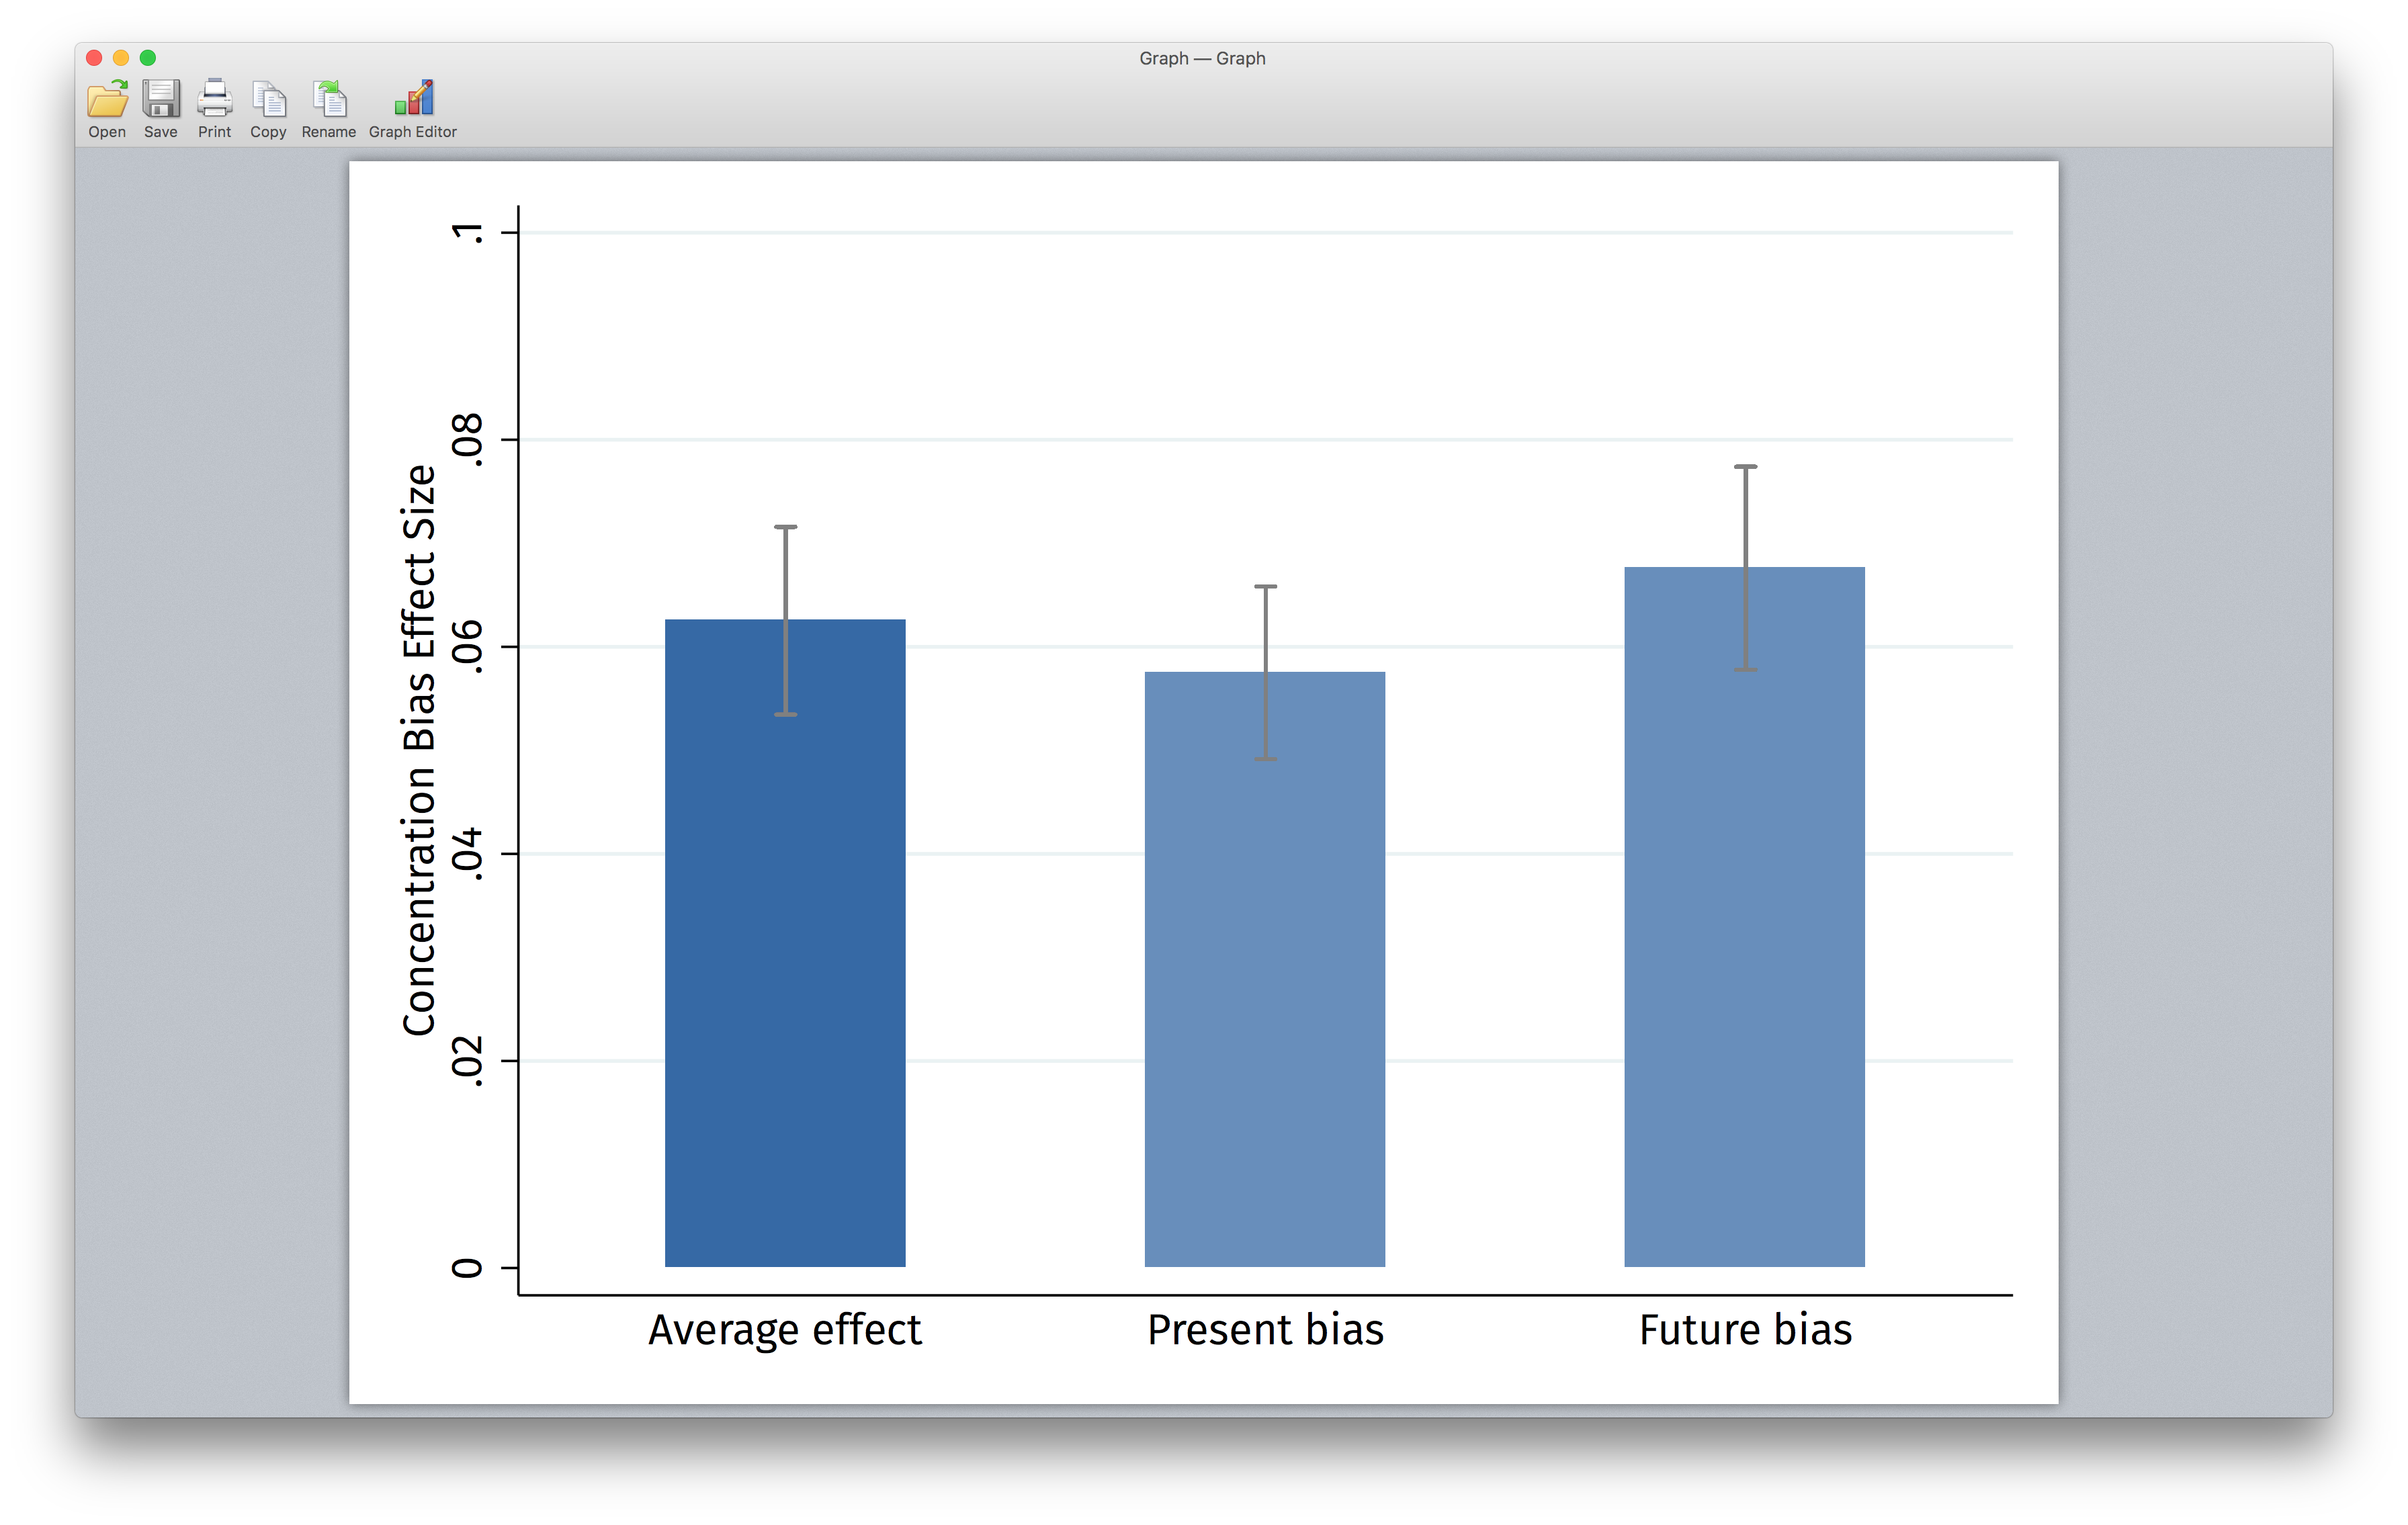
\includegraphics[width=1.643in, trim={3.75in 1.75in 3.75in 2in}, clip]
					{1_Example_Content/Images/average_pb_fb.png} \\
				\centering \footnotesize \sffamily
				$\text{\balA} - \text{\unbalA[\bullet]}$
			\end{minipage}
			\hspace{2pt}
			\begin{minipage}[t]{0.46\textwidth}
				\Large\textbf{B} \textcolor{SpotColor}{\hspace{0.39in} {\small \textbf{Result~2}}} \\[15pt]
				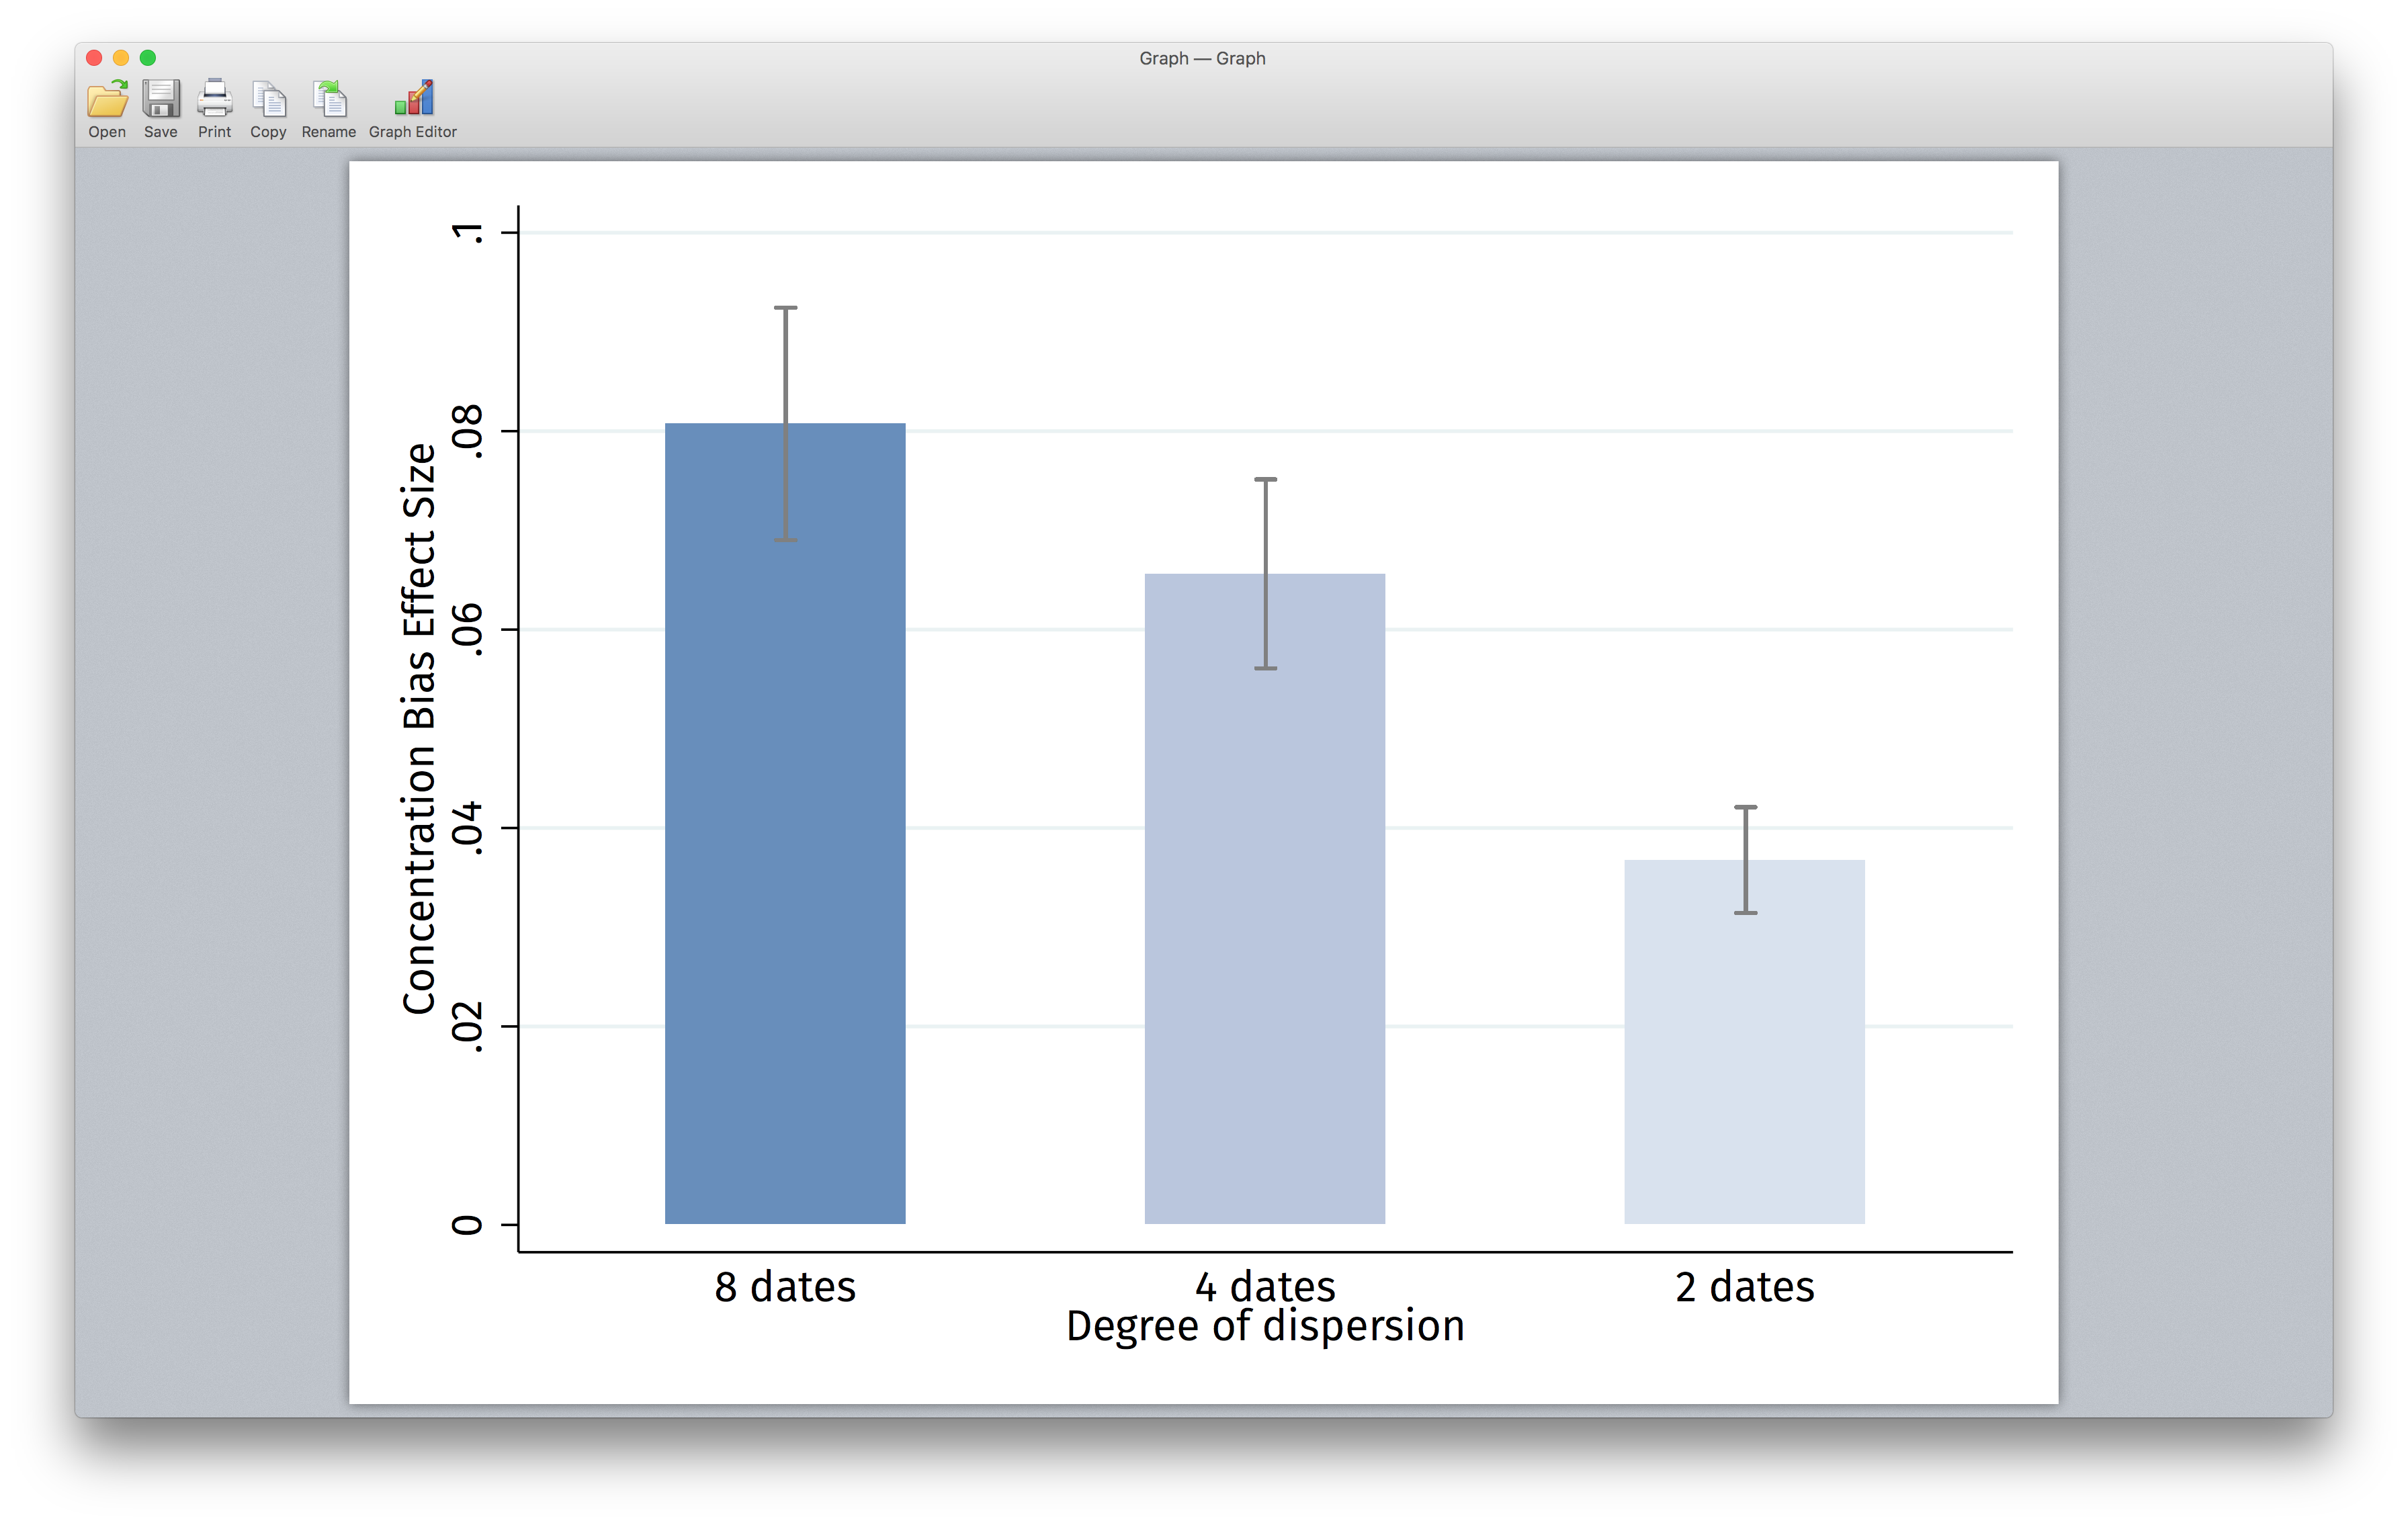
\includegraphics[width=1.710in, trim={3.75in 1.75in 3.75in 2in}, clip]
					{1_Example_Content/Images/average_8_4_2.png} \\
				\centering \footnotesize \sffamily
				$\text{\unbalB[\bullet]} - \text{\balB}$
			\end{minipage} \\
		\end{minipage}
		\caption{%
			\textbf{(A)}~Difference between treatment and control condition. \textbf{(B)}~Heterogeneity.%
		}
	\end{figure}
	
\end{frame}


\begin{frame}{\titleprefix: Main vs. Control Experiment}

	Rule out some alternative explanations \citep{Dertwinkel-Kalt2017}.
	
	\bigskip
	
	\centering
	{\small \alert{Result~3}} \\[15pt]
	% trim={<left> <lower> <right> <upper>}
	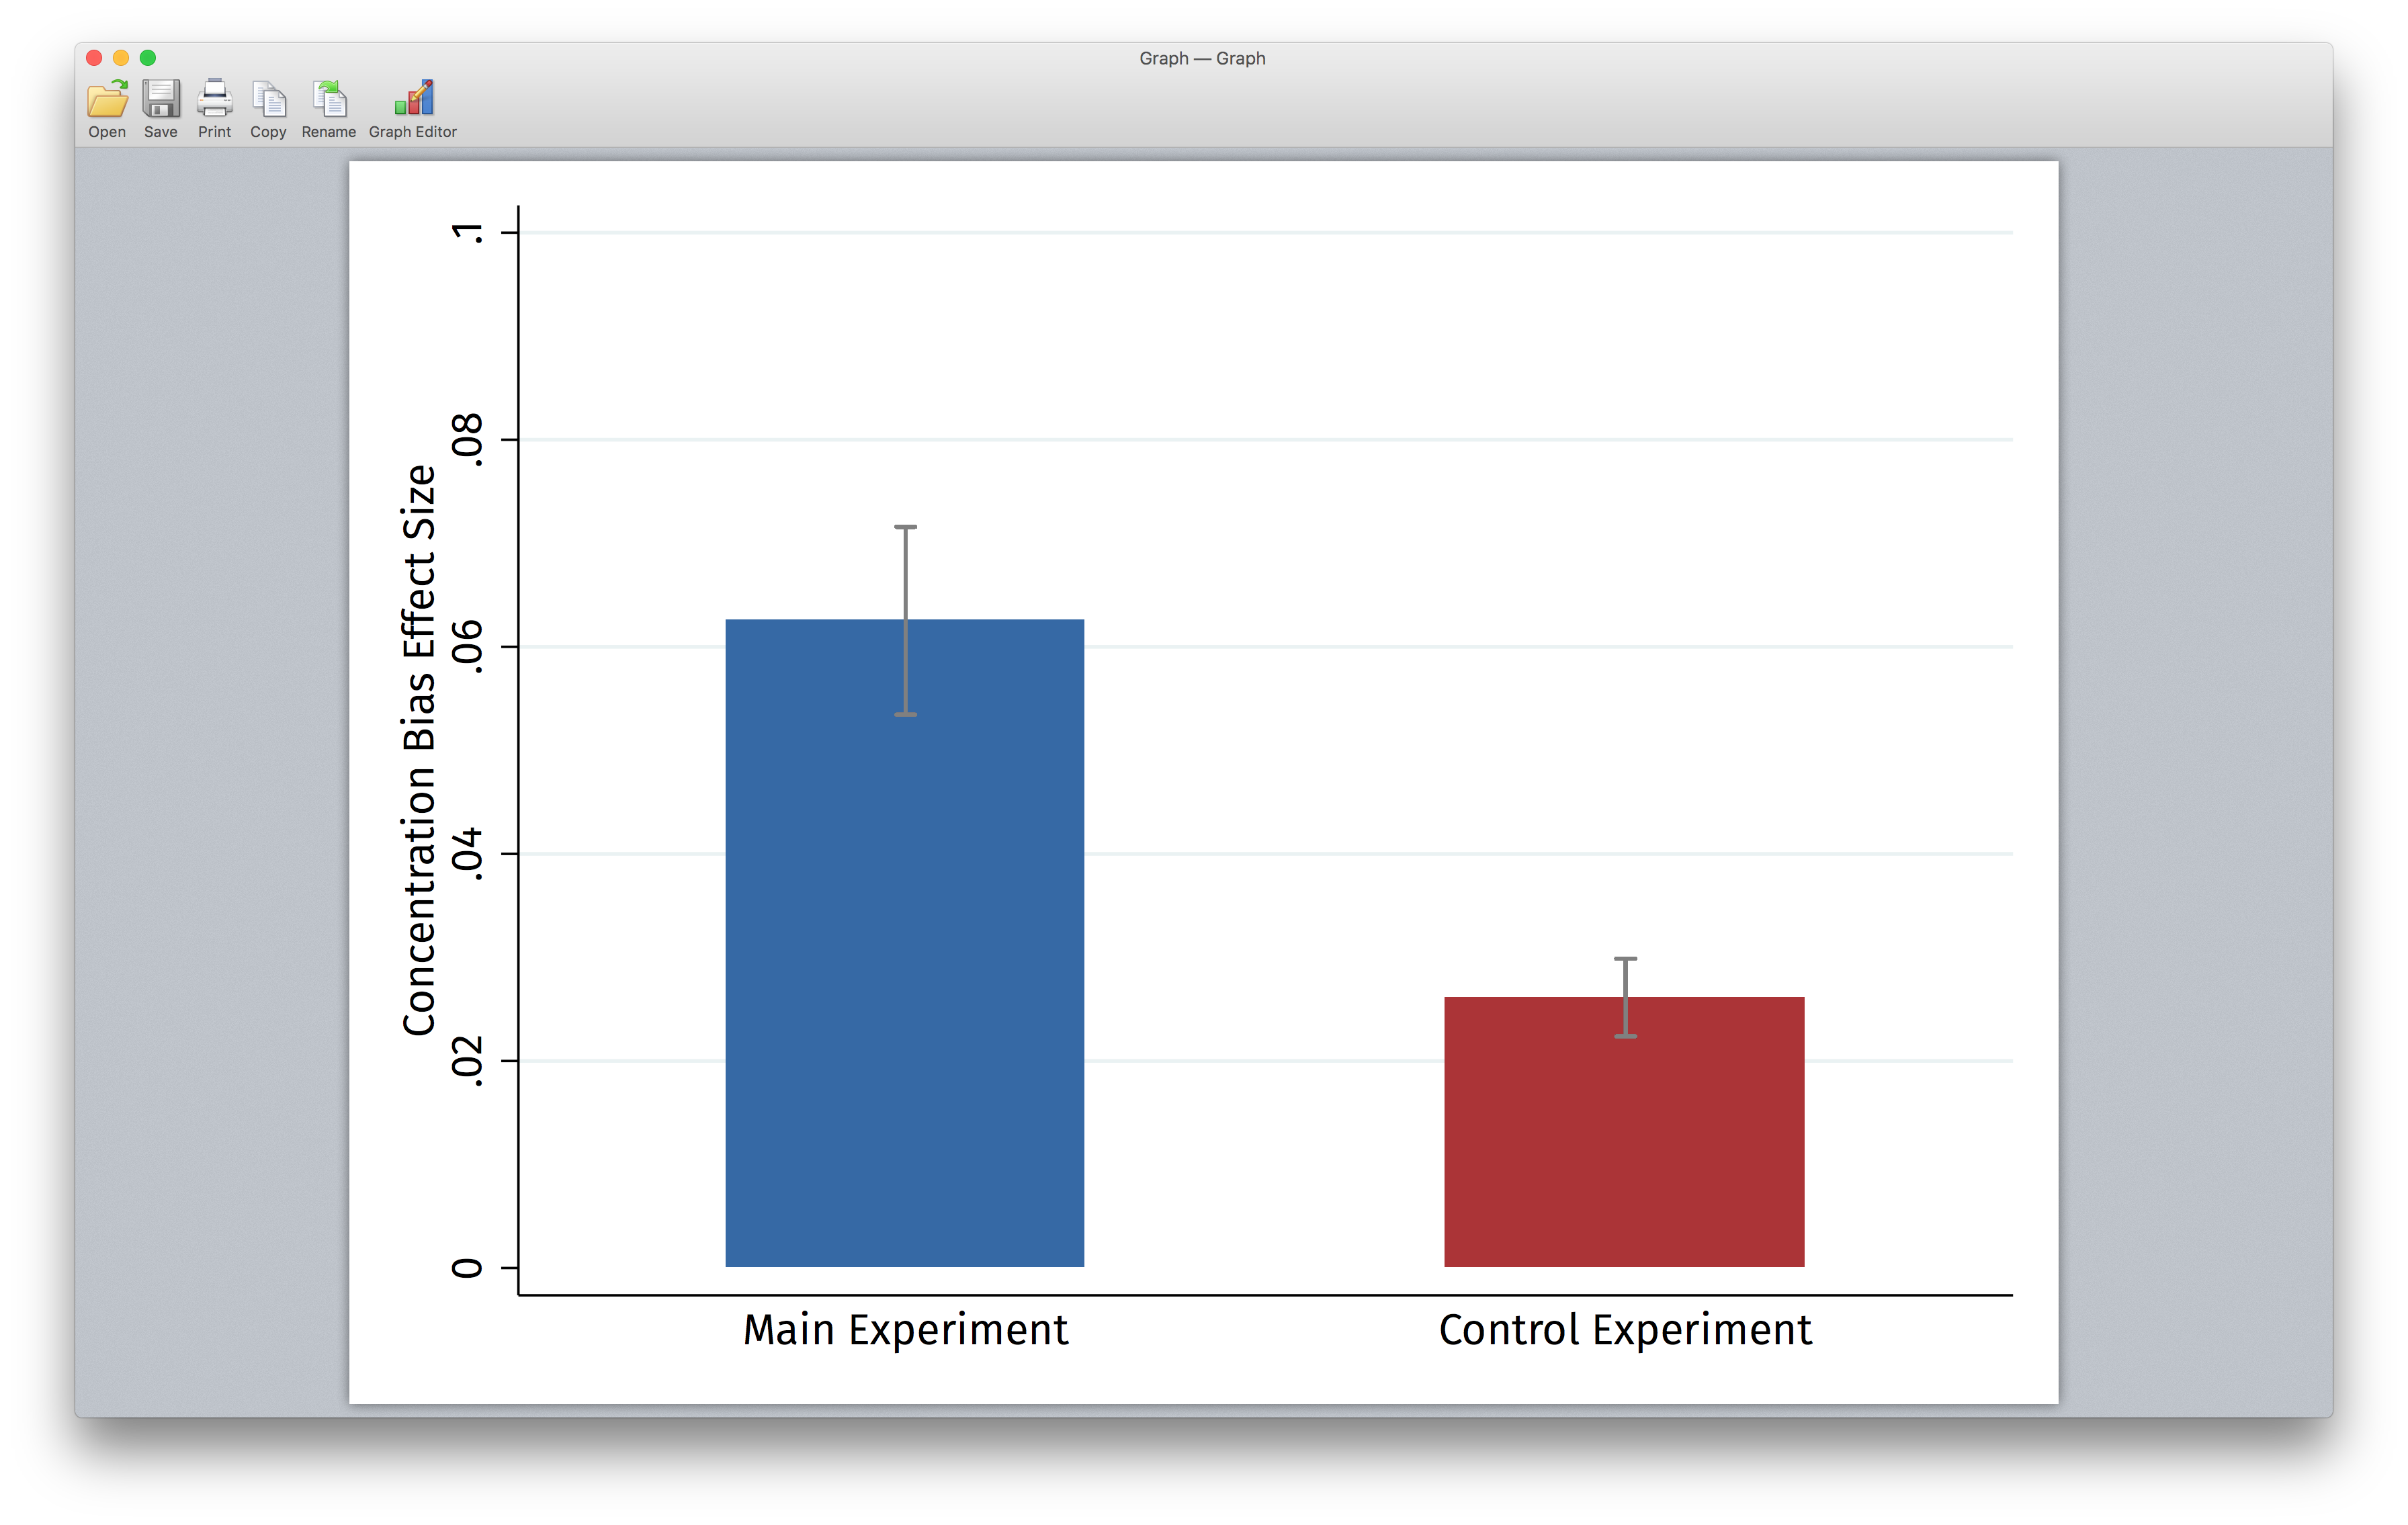
\includegraphics[height=0.5\textheight, trim={3.75in 1.75in 3.75in 2in}, clip]
		{1_Example_Content/Images/average_main_control.png}

\end{frame}


\begin{frame}{\titleprefix: Another \texttt{siunitx} Example Table}

	\begin{table}
	\caption{%
		Example of a~regression table \citep[adapted from][]{Gerhardt2017}.
		Never forget to mention the dependent variable (here, $m_\sim$)!%
	}
	\label{tab:lin_reg_interactions}
	\resizebox*{!}{0.59\textheight}{%
		\mdseries\selectfont
		\footnotesize
\newcolumntype{U}{S[table-format=+1.3, round-mode=places, round-precision=3, table-space-text-pre={**}, table-space-text-post={-**}, round-integer-to-decimal=false]}
\begin{tabularx}
	{\textwidth}
	{@{} L @{\hspace{1.5em}} U @{\hspace{1em}} U @{\hspace{1em}} U @{\hspace{1em}} U @{\hspace{1em}} U @{}}
\toprule
&	{(1)}	&	{(2)}	&	{(3)}	&	{(4)}	&	{(5)} \\
\midrule
Treatment
	&	-0.390	&	-0.228	&	-0.729*	&	-0.449*	&	-0.453**	\\
	&	(+0.352)	&	(-0.205)	&	[+0.377]	&	[-0.245]	&	{\{}+0.204{\}}	\\
Female
	&	0.948***	&	0.0607	&	0.188	&	0.305	&	0.385*	\\
	&	(0.354)	&	(0.233)	&	(0.372)	&	(0.226)	&	(0.222)	\\
$\text{Female} \times \text{Treatment}$
	&	0.169	&	0.251	&	0.892*	&	0.454	&	0.439	\\
	&	(0.514)	&	(0.325)	&	(0.533)	&	(0.341)	&	(0.307)	\\
Final high school grade
	&	-0.101	&	0.0132	&	0.0759	&	0.117	&	0.0394	\\
	&	(0.198)	&	(0.144)	&	(0.224)	&	(0.146)	&	(0.133)	\\
Trait self-control
	&	-0.0156	&	0.00214	&	-0.0160	&	-0.000122	&	-0.00678	\\
	&	(0.0162)	&	(0.00994)	&	(0.0147)	&	(0.0104)	&	(0.00935)	\\
Constant
	&	2.357***	&	1.512***	&	-0.322	&	2.158***	&	1.437***	\\
	&	(0.239)	&	(0.144)	&	(0.265)	&	(0.161)	&	(0.152)	\\
\midrule
Observations
	&	{303}	&	{289}	&	{295}	&	{304}	&	{1191}	\\
$R^2$
	&	0.057	&	0.008	&	0.039	&	0.043	&	0.024	\\
\midrule
$\text{Treatment} \times \text{(1 + Female)}$
	&	-0.221	&	0.0228	&	0.163	&	0.00435	&	-0.0138	\\
$p_F[\text{Treatment} \times {}$ \newline\hspace{12pt}$(1 + \text{Female}) = 0]$
	&	0.327	&	0.00767	&	0.192	&	0.000314	&	0.00343	\\
\bottomrule
\addlinespace
\multicolumn{6}{@{} p{\textwidth} @{}}{%
	\textit{Notes:} Dependent variable: $m_\sim$. Robust standard errors (cluster-corrected for column~5) in parentheses. ***\,${p < 0.01}$, **\,${p < 0.05}$, *\,${p < 0.1}$. Missing observations (${N < 308}$) due to exclusion of trials in which subjects behaved irrationally (i.e., chose a~dominated option). The regressors Final high school grade and Trait self-control are mean-centered.
}
\end{tabularx}
	}
	\end{table}

\end{frame}


\begin{frame}{\titleprefix: Yet Another \texttt{siunitx} Example Table}

	\begin{table}
		\caption{Figure grouping via \texttt{siunitx} in a~table.}
		\begin{tabular}
	{ @{}
	  S[table-format=+1.3, table-space-text-pre={**}, table-space-text-post={-**}]
	  S[table-format=+1.5, table-space-text-pre={**}, table-space-text-post={-**}]
	  S[table-format=+6.3, table-space-text-pre={**}, table-space-text-post={-**}]
	  @{}
	}
	\toprule
	{(1)}	&  {(2)}		& {(3)}\\
	\midrule
	-0.100*	& -0.10001*	& -123456.444*** \\
	(2.871) & (2.87123)		& [+50000.123] \\
	\bottomrule
\end{tabular}
	\end{table}

\end{frame}


\section{Discussion}


\begin{frame}{\titleprefix}

	\begin{itemize}[<+->]
		\item The latex exhibits a neutral, acid, or alkaline reaction, depending on the plant from which it was obtained.
		\item The latex is therefore usually allowed to coagulate on the tree \citep{Koszegi2013}.
			\begin{itemize}
				\item<.->[$\Rightarrow$] The latex, which is usually coagulated by standing or by heating, is obtained from incisions.
			\end{itemize}
		\item See also \cite{Bordalo2013, Dohmen2012}.
	\end{itemize}	

\end{frame}


\begin{frame}{\titleprefix: Conclusion}

	\begin{itemize}
		\item When exposed to air, the latex gradually undergoes putrefactive changes accompanied by coagulation.
		\item The addition of a small quantity of ammonia or of formalin to some latices has the effect of preserving them.
		\item There is, however, reason to believe the following.
		\item The coagulation of latex into rubber is not mainly of this character.
	\end{itemize}

\end{frame}


\begin{frame}{\titleprefix: An Automated Animation}

The automated transition to the next slide (=~page in the PDF document) only works in full-screen mode.
\begin{itemize}
	\item The feature is available in Adobe Acrobat and Acrobat Reader.
	\item Unfortunately, it is (currently, \today) not available in macOS Preview, Skim, and SumatraPDF.
\end{itemize}
\transduration{0.25}%
\only<12>{\transduration{}}\hypertarget<1>{animation_start}{}%
\foreach \n [evaluate=\n as \angle using \n * 30] in {0, ..., 12}{
	\only<\n>{
		\begin{figure}
			\begin{tikzpicture}
				\draw[draw=none, use as bounding box](-1, 0) rectangle (1, 2);
				\filldraw[fill=SpotColor, draw=none] (0,1) -- (0,2) arc (90:90-\angle:1cm) -- cycle;
			\end{tikzpicture}
			\caption{Step~\n---Angle: \angle\textdegree}
		\end{figure}
	}
}%
\vspace{-\bigskipamount}
\hyperlink<12>{animation_start}{\beamerreturnbutton{Back to the start}}
		
\end{frame}


\begin{frame}[allowframebreaks]{\titleprefix: Testing the \texttt{allowframebreaks} option}

Let's test automatic numbering with the \texttt{allowframebreaks} option.

On this slide, \textbf{no} number should be included in the frame title.

\end{frame}


\begin{frame}[allowframebreaks]{\titleprefix: Testing the \texttt{allowframebreaks} Option}

\renewcommand{\blindmarkup}[1]{\emph{#1}}

Let's test automatic numbering with the \texttt{allowframebreaks} option.

On this slide, ``(1/3)'' should appear in the frame title.

\blindtext

\parstart{\framebreak}
\Blindtext[2]

\end{frame}


\section{Math ``Torture'' Test}


\begin{frame}[allowframebreaks]{\insertsection}
	
Most of the following examples are taken from \textit{The \TeX book} \citep[][see \url{https://ctan.org/pkg/texbook}]{Knuth1984} and were adapted for \LaTeX\ from Karl Berry's torture test for plain \TeX\ math fonts.

\noindent $x + y - z$, \quad $x + y * z$, \quad $z * y / z$, \quad 
$(x+y)(x-y) = x^2 - y^2$, 

\noindent $x \times y \cdot z = [x\, y\, z]$, \quad $x\circ y \bullet z$, \quad
$x\cup y \cap z$, \quad $x\sqcup y \sqcap z$, \quad

\noindent $x \vee y \wedge z$, \quad $x\pm y\mp z$, \quad
$x=y/z$, \;\; $x:=y$, \;\; $x\le y \ne z$, \;\; $x \sim y \simeq z$
$x \equiv y \nequiv z$, \;\; $x\subset y \subseteq z$

\noindent $\sin2\theta=2\sin\theta\cos\theta$, \quad
$\hbox{O}(n\log n\log n)$, \quad
$\Pr(X>x)=\exp(-x/\mu)$,

\noindent $\bigl(x\in A(n)\bigm|x\in B(n)\bigr)$, \quad
$\bigcup_n X_n\bigm\|\bigcap_n Y_n$

% page 178

\noindent In-text matrices $\binom{1\,1}{0\,1}$ and $\bigl(\genfrac{}{}{0pt}{}{a}{1}\genfrac{}{}{0pt}{}{b}{m}\genfrac{}{}{0pt}{}{c}{n}\bigr)$.

\framebreak
% page 142

$$a_0+\frac1{\displaystyle a_1 +
	{\strut \frac1{\displaystyle a_2 +
			{\strut \frac1{\displaystyle a_3 +
					{\strut \frac1{\displaystyle a_4}}}}}}}$$
% page 143
$$\binom{p}{2}x^2y^{p-2} - \frac1{1 - x}\frac{1}{1 - x^2}
=
\frac{a+1}{b}\bigg/\frac{c+1}{d}.$$
%% page 145
$$\sqrt{1+\sqrt{1+\sqrt{1+\sqrt{1+\sqrt{1+x}}}}}$$
$$\sqrt[n]{1+\sqrt[k]{1+\sqrt[5]{1+\sqrt[4]{1+\sqrt[3]{1+x}}}}}$$

\framebreak
%% page 147

$$\left(\frac{\partial^2}{\partial x^2} + \frac{\partial^2}{\partial y^2}\right)
\bigl|\varphi(x+\mathup{i}y)\bigr|^2=0$$

%% page 149

% $$\pi(n)=\sum_{m=2}^n\left\lfloor\biggl(\sum_{k=1}^{m-1}\bigl
% \lfloor(m/k)\big/\lceil m/k\rceil\bigr\rfloor\biggr)^{-1}\right\rfloor.$$

$$\pi(n)=\sum_{m=2}^n\left\lfloor\Biggl(\sum_{k=1}^{m-1}\bigl
\lfloor(m/k)\big/\lceil m/k\rceil\bigr\rfloor\Biggr)^{-1}\right\rfloor.$$

% page 168

$$\int_0^\infty \frac{t - \mathup{i} b}{t^2 + b^2}e^{\mathup{i}at}\,\mathup{d}t=e^{ab}E_1(ab), \quad
a,b > 0.$$

% page 176

$$\mathbf{A} \coloneqq \begin{pmatrix}x-\lambda&1&0\\
0&x-\lambda&1\\
0&0&x-\lambda\end{pmatrix}.$$

\framebreak

$$\left\lgroup\begin{matrix}a&b&c\\ d&e&f\\\end{matrix}\right\rgroup
\left\lgroup\begin{matrix}u&x\cr v&y\cr w&z\end{matrix}\right\rgroup$$
% page 177
$$\mathbf{A} = \begin{pmatrix}a_{11}&a_{12}&\ldots&a_{1n}\\
a_{21}&a_{22}&\ldots&a_{2n}\\
\vdots&\vdots&\ddots&\vdots\\
a_{m1}&a_{m2}&\ldots&a_{mn}\end{pmatrix}$$
$$\mathbf{M}=\bordermatrix{&C&I&C'\cr
	C&1&0&0\cr I&b&1-b&0\cr C'&0&a&1-a}$$

\framebreak
%% page 186

$$\sum_{n=0}^\infty a_nz^n\quad\hbox{converges if}\quad
|z|<\Bigl(\limsup_{n\to\infty}\root n\of{|a_n|}\,\Bigr)^{-1}.$$

$$\frac{f(x+\mathup{\Delta} x)-f(x)}{\mathup{\Delta} x}\to f'(x)
\qquad \hbox{as $\mathup{\Delta} x\to0$.}$$

$$\|u_i\|=1,\qquad u_i\cdot u_j=0\quad\hbox{if $i\ne j$.}$$

%% page 191

$$\hbox{The confluent image of}\quad
\begin{Bmatrix}\hbox{an arc}\hfill\\\hbox{a circle}\hfill\\
\hbox{a fan}\hfill\\\end{Bmatrix}
\quad\hbox{is}\quad
\begin{Bmatrix}\hbox{an arc}\hfill\\
\hbox{an arc or a circle}\hfill\\
\hbox{a fan or an arc}\hfill\end{Bmatrix}.$$

\framebreak
%% page 191

\begin{align*}
T(n)\le T(2^{\lceil\lg n\rceil})
&\le c(3^{\lceil\lg n\rceil}-2^{\lceil\lg n\rceil})\\
&<3c\cdot3^{\lg n}\\
&=3c\,n^{\lg3}.
\end{align*}
%\begin{align*}
%\left\{%
%\begin{gathered}\alpha&=f(z)\\ \beta&=f(z^2)\\ \gamma&=f(z^3)
%\end{gathered}
%\right\}
%\qquad
%\left\{%
%\begin{gathered}
%x&=\alpha^2-\beta\\ y&=2\gamma
%\end{gathered}
%\right\}%
%\end{align*}
%$$\left\{
%\begin{align}
%\alpha&=f(z)\cr \beta&=f(z^2)\cr \gamma&=f(z^3)\\
%%\end{align}
%\right\}
%\qquad
%\left\{
%%\begin{align}
%x&=\alpha^2-\beta\cr y&=2\gamma\\
%\end{align}
%\right\}.$$
%%% page 192
\begin{align*}
\begin{aligned}
(x+y)(x-y)&=x^2-xy+yx-y^2\\
&=x^2-y^2\\
(x+y)^2&=x^2+2xy+y^2.
\end{aligned}
\end{align*}

\framebreak
%% page 192

\begin{align*}
\begin{aligned}
\left( \int\limits_{-\infty}^\infty \mathup{e}^{-x^2}\,\mathup{d}x \right)^2
&=\int_{-\infty}^\infty\int_{-\infty}^\infty \mathup{e}^{-(x^2+y^2)}\,\mathup{d}x\,\mathup{d}y\\
&=\int_0^{2\piup}\int_0^\infty \mathup{e}^{-r^2}\,\mathup{d}r\,\mathup{d}\theta\\
&=\int_0^{2\piup}\biggl(\mathup{e}^{-\frac{r^2}{2}}
\biggl|_{r=0}^{r=\infty}\,\biggr)\,\mathup{d}\theta\\
&=\piup.
\end{aligned}
\end{align*}

\framebreak
%% page 197

$$\prod_{k\ge0}\frac{1}{(1-q^kz)}=
\sum_{n\ge0}z^n\bigg/\!\!\prod_{1\le k\le n}(1-q^k).$$

$$\sum_{\substack{\scriptstyle 0< i\le m\\\scriptstyle0<j\le n}}p(i,j) \,\ne
%
% $$\sum_{i=1}^p \sum_{j=1}^q \sum_{k=1}^r a_{ij} b_{jk} c_{ki}$$
%
\sum_{i=1}^p \sum_{j=1}^q \sum_{k=1}^r a_{ij} b_{jk} c_{ki} \,\ne
%
\sum_{\substack{\scriptstyle 1\le i\le p \\ \scriptstyle 1\le j\le q\\
		\scriptstyle 1\le k\le r}} a_{ij} b_{jk} c_{ki}$$

\framebreak

$$\max_{1\le n\le m}\log_2P_n \quad \hbox{and} \quad
\lim_{x\to0}\frac{\sin x}{x}=1$$
Inline math:
$\max_{1\le n\le m}\log_2P_n \quad \hbox{and} \quad
\lim_{x\to0}\frac{\sin x}{x}=1$
$$p_1(n)=\lim_{m\to\infty}\sum_{\nu=0}^\infty\bigl(1-\cos^{2m}(\nu!^n\piup/n)\bigr)$$
Inline math:
$p_1(n)=\lim_{m\to\infty}\sum_{\nu=0}^\infty\bigl(1-\cos^{2m}(\nu!^n\piup/n)\bigr)$

\end{frame}




%%%%%%%%%%%%%%%%%%
%%  REFERENCES  %%
%%%%%%%%%%%%%%%%%%


\section{\refname}
%\renewcommand\bibsection{}
%	% To prevent ``References'' from appearing twice in the navigation bar

\begin{frame}[allowframebreaks]{\insertsection}

	\begin{refcontext}[sorting=nyt]
		% Sort BIBLIOGRAPHY by alphabet (while CITATIONS are sorted by year)
	\printbibliography[heading=none]
	\end{refcontext}

	%% Only when using BibTeX instead of BibLaTeX ==>
	%\bibliographystyle{0_0_Preamble/aea_doi_url_href}
	%\bibliography{Library}
	%% <==
	
\end{frame}




%%%%%%%%%%%%%%%%
%%  APPENDIX  %%
%%%%%%%%%%%%%%%%


\begin{appendix}


\section[Appendix\newline \textmd{Backup Slides}]{Appendix}


\begin{frame}[label=model]

	\frametitle{\insertsection: Modeling Concentration Bias}
	
	Subjects consider a sequences of consequences $\boldsymbol{c}$ from choice set $\boldsymbol{C}$.
	
	%Focusing theory augments discounted utility (constant, hyperbolic, \dots) through an~additional weight \highlight{$g[\cdot]$} on the instantaneous utility function.
	\begin{itemize}
	
	\item \alert{Standard discounted utility:}
		Suppose that the instantaneous utility function $u$ satisfies ${u'>0}$ and ${u''\leq 0}$, and that earlier consequences are preferred over later consequences of the same magnitude, i.e., ${D(t)\leq 1}$:
	\item[] ${U}(\boldsymbol{c}\phantom{, \boldsymbol{C}}) \coloneqq
		\sum_{t=1}^{T} \phantom{g_t} D(t)\,u(c_t)$, \quad where, e.g., \quad $D(t) = \delta^t$  or $D(t) = \frac{1}{1 + k\,t}$. %$\beta \delta^t$.
	\medskip
	\item \only<1->{\alert{Focusing model \citep{Koszegi2013}:}}
	\item[]<1-> $\tilde{U}(\boldsymbol{c}\highlight{, \boldsymbol{C}}) \coloneqq \sum_{t=1}^{T} \highlight{g_t}\,D(t)\,u(c_t)$, \quad where \\[3pt]
		\highlight{$g_t \equiv % g[\Delta_t(C)]$, $\Delta_t(C) =
		g[\max_{\boldsymbol{c}'\in \boldsymbol{C}} %D(t) 
		u(c'_t) - \min_{\boldsymbol{c}'\in \boldsymbol{C}} %D(t) 
		u(c'_t)]$}
		\smallskip
		\begin{itemize}
			\item<1-> Weighting function \highlight{$g[\cdot]$} increases in difference of maximum and minimum possible utility at a~point in time.
			\item<1-> Subjects overweight intertemporal consequences with a greater range.
			%\item<3-> Subjects overweight intertemporal consequences with a greater range 
		\end{itemize}
	\end{itemize}

\end{frame}


\end{appendix}